\subsubsection{Total number of collisions}\label{subsubsec:hd2krcollisions}

For the total number of collisions we get a very low unexplained variation
(\(0.52\%\)). The broadcast radius accounts for the \(78.81\%\) of the variation
and it is the dominant factor. Also the maximum relay delay and the maximum
number of copies have an impact on this index of the \(6.32\%\) and the
\(5.56\%\) respectively.

From the performance plot shown in \figref{subfig:hdperfcollisionsR} we can see
that reducing the broadcast radius we can obtain much lower values for the
number of collisions: less than 1000 with \(R\!=\!10m\) and always above 2000
and up to over 5500 with \(R\!=\!20m\). In \figref{subfig:hdperfcollisionsD} we
show that an higher maximum relay delay means a lower number of collisions: this
happens because, with a larger \(\max(\delta)\), different users relay their
message in different slots more often. Of course, also the maximum number of
copies has an impact on the number of collisions, as shown in
\figref{subfig:hdperfcollisionsm}, since an higher value for this factor means a
higher number of retransmissions, especially in more crowded areas of the
floorplan where there are more users that relay their message to others.

\begin{figure}[htb]
	\centering
	\begin{subfigure}[b]{0.38\textwidth}
		\centering
		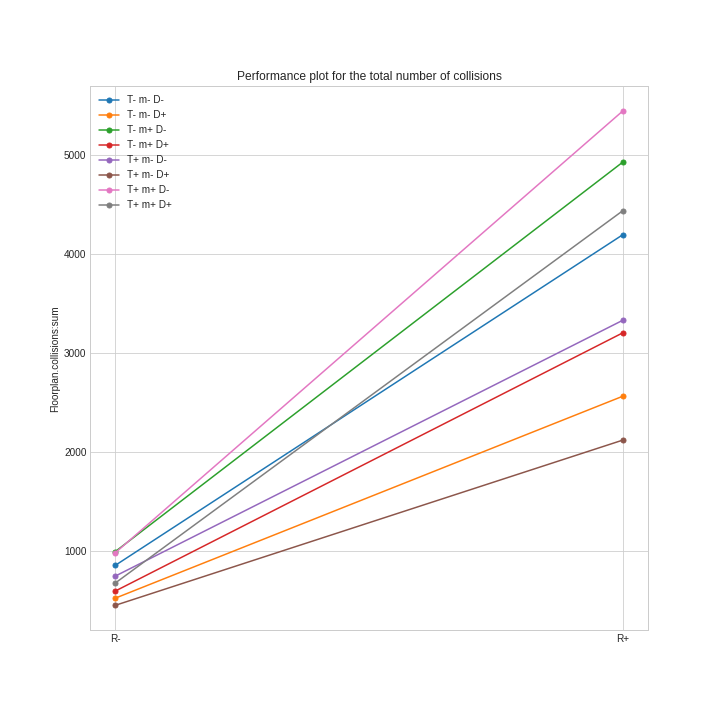
\includegraphics[width=\textwidth]{img/hd/collisions-R-perfplot}
		\caption{The broadcast radius has an huge impact on the total
		number of collisions}\label{subfig:hdperfcollisionsR}
	\end{subfigure}
	\begin{subfigure}[b]{0.38\textwidth}
		\centering
		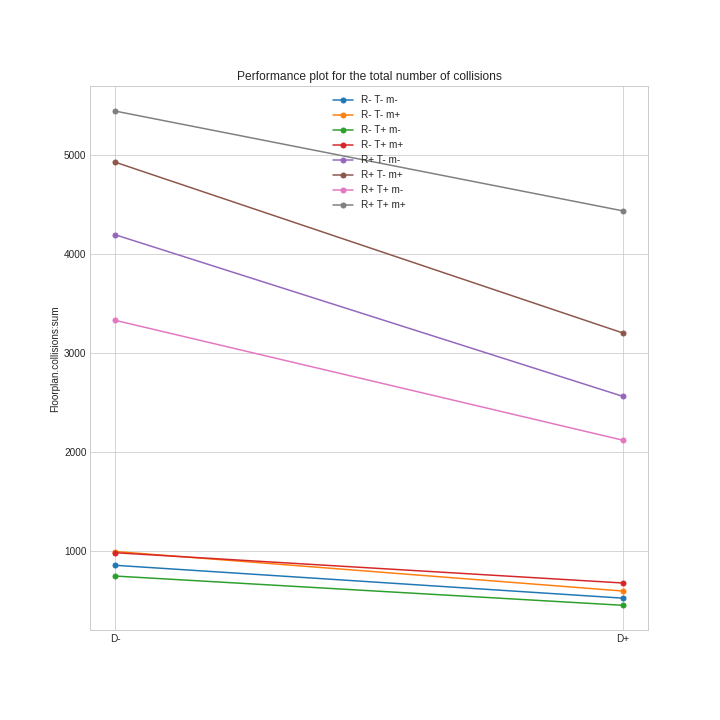
\includegraphics[width=\textwidth]{img/hd/collisions-D-perfplot}
		\caption{Increase the maximum relay delay to reduce the total
		number of collisions}\label{subfig:hdperfcollisionsD}
	\end{subfigure}\\
	\begin{subfigure}[b]{0.37\textwidth}
		\centering
		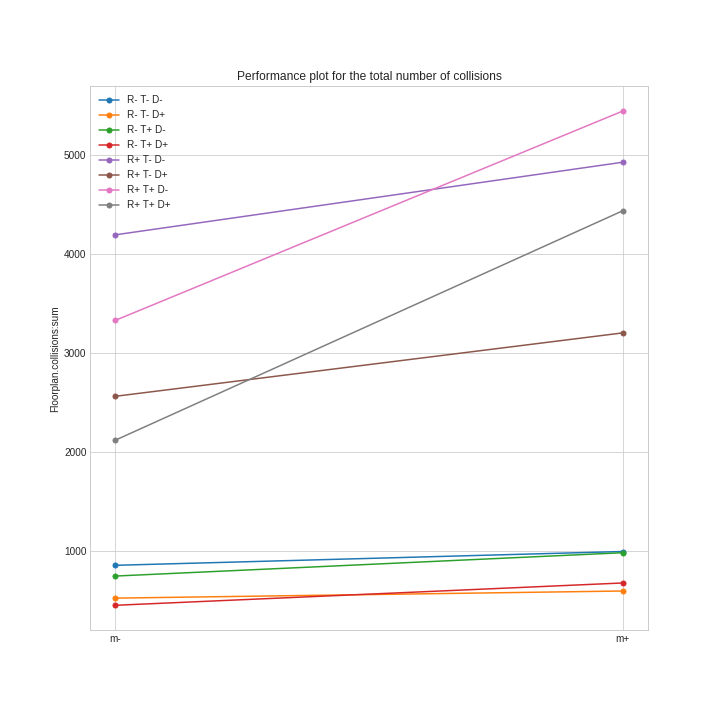
\includegraphics[width=\textwidth]{img/hd/collisions-m-perfplot}
		\caption{Decrease the maximum number of copies to decrease the
		total number of collisions}\label{subfig:hdperfcollisionsm}
	\end{subfigure}
	\caption{Performance plots for the total number of
	collisions}\label{fig:hdperfcollisions}
\end{figure}

Probably we do not want to reduce the broadcast radius just to reduce the total
number of collisions. This performance index is in fact usually less important
than the others: if we have ``good'' results for the coverage, the broadcast
time and the energy efficiency of the network, even an high number of collisions
would be probably acceptable. So we should probably evaluate to increase the
maximum relay delay and the maximum number of copies to reduce the number of
collisions: this should indirectly affect the energy efficiency by reducing the
total number of messages sent, especially if we decrease the \code{maxCopies}
parameter.
